%%%%%%%%%%%%%%%%%%%%%%%%%%%%%%%%%%%%%%%%%
% University/School Laboratory Report
% LaTeX Template
% Version 3.1 (25/3/14)
%
% This template has been downloaded from:
% http://www.LaTeXTemplates.com
%
% Original author:
% Linux and Unix Users Group at Virginia Tech Wiki 
% (https://vtluug.org/wiki/Example_LaTeX_chem_lab_report)
%
% License:
% CC BY-NC-SA 3.0 (http://creativecommons.org/licenses/by-nc-sa/3.0/)
%
%%%%%%%%%%%%%%%%%%%%%%%%%%%%%%%%%%%%%%%%%

%----------------------------------------------------------------------------------------
%	PACKAGES AND DOCUMENT CONFIGURATIONS
%----------------------------------------------------------------------------------------

\documentclass{article}

\usepackage[version=3]{mhchem} % Package for chemical equation typesetting
\usepackage{siunitx} % Provides the \SI{}{} and \si{} command for typesetting SI units
\usepackage{graphicx} % Required for the inclusion of images
\usepackage{natbib} % Required to change bibliography style to APA
\usepackage{amsmath} % Required for some math elements 
\usepackage[utf8]{inputenc}
\usepackage{tikz,pgfplots}
\usepackage[letterpaper, margin=1in]{geometry}
\usepackage{float}
\usepackage{enumitem}

\pagenumbering{arabic}

\setlength\parindent{0pt} % Removes all indentation from paragraphs

\renewcommand{\labelenumi}{\alph{enumi}.} % Make numbering in the enumerate environment by letter rather than number (e.g. section 6)

%\usepackage{times} % Uncomment to use the Times New Roman font

% for some tables
\newcommand{\specialcell}[2][c]{%
  \begin{tabular}[#1]{@{}c@{}}#2\end{tabular}}
  
\providecommand{\e}[1]{\ensuremath{\times 10^{#1}}}
%----------------------------------------------------------------------------------------
%	DOCUMENT INFORMATION
%----------------------------------------------------------------------------------------

%\title{Determination of the Atomic \\ Weight of Magnesium \\ CHEM 101} % Title

%\author{John \textsc{Smith}} % Author name

%\date{\today} % Date for the report

\begin{document}

%\maketitle % Insert the title, author and date

% If you wish to include an abstract, uncomment the lines below
% \begin{abstract}
% Abstract text
% \end{abstract}

%----------------------------------------------------------------------------------------
%	SECTION 1
%----------------------------------------------------------------------------------------

\section{Objective}

To use the Rockwell and Brinell tests to create deformations and compare results of various metals and alloys. These tests will help better understand how mechanical stress and strain behave.

% If you have more than one objective, uncomment the below:
%\begin{description}
%\item[First Objective] \hfill \\
%Objective 1 text
%\item[Second Objective] \hfill \\
%Objective 2 text
%\end{description}

\section{Experimental Procedures}
\subsection{Rockwell hardness test}
We placed a piece of metal into the machine and turned the crank shaft near the bottom of the machine until the piece locked into place and the small arrow on the dial was pointing towards the black dot. At this point there is a minor load of 10 kg being applied to the material. We then twisted the dial adjustment shaft directly under the crank shaft to zero the machine. Zeroing the machine meant aligning the long arrow with the black 0 mark on the dial. Then we pushed down on the handle to apply the 60 kg major load and started a 15 second timer. After the 15 seconds we pulled forward on the handle located on the bottom right side of the machine to release the load. We measured the results using the black – not red – tick marks on the dial and then twisted the crank shaft to release the material.

\subsection{Brinell hardness test}
We placed the piece in the machine and used a similar crank shaft to lock the piece into place. Then we turned the pressure knob near the top of the machine until it was just tight enough where it would not come loose by itself. Then we began pulling the lever and pumping the pressure up to the required position (500 kg or 3000 kg) and starting our time for the required time (30 seconds or 15 seconds). We knew to start the timer right when the ball supporting the weights on the machine lifted up and started floating.

\begin{figure}[H]
\caption{schematic of rubber plate used}
\centering
\begin{tikzpicture}
\node at (5,5) {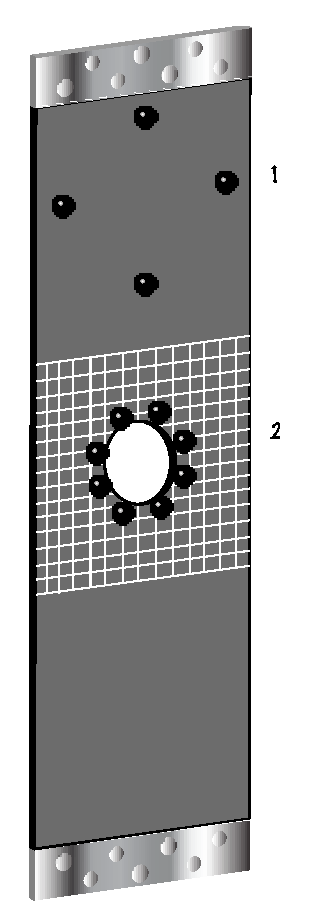
\includegraphics[width=100pt]{diagram11.pdf}};
\draw [red,<->] (3.9,7.6) -- (5.8,7.9);
\node [red] at (4.4,8) {$X_1$};
\draw [blue,<->] (4.75,6.8) -- (4.75,8.5);
\node [blue] at (5.1,7.4) {$Y_1$};

\draw [red,<->] (4.5,5.5) -- (4.9,5.55);
\node [red] at (4.7,5.9) {\textbf{$X_2$}};
\draw [blue,<->] (5.2,4.8) -- (5.2,5.3);
\node [blue] at (5.6,5) {\textbf{$Y_2$}};
\end{tikzpicture}
\end{figure}

 \subsection{Stress Concentration Analysis}
Refer to Figure 1 for reference. We initially measured the width and depth of the rubber plate at the top of the plate and at the bottom near the hole. Then we measured $x_1 \,y_1 \,x_2 \,y_2$. We then consecutively added 10 lbs to the load of the rubber sheet and remeasured $x_1 \,y_1 \,x_2 \,y_2$ again after every 10 lbs.

%----------------------------------------------------------------------------------------
%	SECTION 2
%----------------------------------------------------------------------------------------

\section{Experimental Results}
\begin{figure}[H]
\centering
\begin{tabular}{c || c | c | c | c | c | c }
Material & Trial \# & \specialcell{Major load \\(kg)}& \specialcell{Minor load \\(kg)} & \specialcell{Scale \\(0.002 mm)} & Hardness & \specialcell{Conversion to \\ Brinell} \\ \hline
 & 1 & 60 & 10 & Rockwell A & 52.6 & 167 \\ 
Mild Steel & 2 & 60 & 10 & Rockwell A & 52.0 & 164 \\ 
 & 3 & 60 & 10 & Rockwell A & 52.0 & 164 \\
 & average & 60 & 10 & Rockwell A & 52.2 & 164\\ \hline
 
  & 1 & 60 & 10 & Rockwell A & 55.9 & 191 \\ 
Stainless Steel & 2 & 60 & 10 & Rockwell A & 53.5 & 173 \\ 
 & 3 & 60 & 10 & Rockwell A & 54.5 & 179 \\
 & average & 60 & 10 & Rockwell A & 54.6 & 180\\ \hline
 
  & 1 & 60 & 10 & Rockwell A & 37.0 & 88 \\ 
Brass & 2 & 60 & 10 & Rockwell A & 37.5 & 90 \\ 
 & 3 & 60 & 10 & Rockwell A & 37.9 & 91 \\
 & average & 60 & 10 & Rockwell A & 37.5 & 90\\ \hline
 
   & 1 & 60 & 10 & Rockwell A & 38.9 & 94 \\ 
Aluminum & 2 & 60 & 10 & Rockwell A & 39.0 & 94 \\ 
 & 3 & 60 & 10 & Rockwell A & 38.0 & 91 \\
 & average & 60 & 10 & Rockwell A & 38.6 & 92\\ \hline
 
   & 1 & 60 & 10 & Rockwell A & 27.0 & 68 \\ 
Copper 0.250 & 2 & 60 & 10 & Rockwell A & 25.8 & 66 \\ 
 & 3 & 60 & 10 & Rockwell A & 29.1 & 72 \\
 & average & 60 & 10 & Rockwell A & 27.3 & 69\\ \hline
 
   & 1 & 60 & 10 & Rockwell A & 32.0 & -- \\ 
Copper 0.230 & 2 & 60 & 10 & Rockwell A & 31.1 & -- \\ 
 & 3 & 60 & 10 & Rockwell A & 30.6 & -- \\
 & average & 60 & 10 & Rockwell A & 31.2 & --\\ \hline
 
   & 1 & 60 & 10 & Rockwell A & 31.9 & -- \\ 
Copper 0.156 & 2 & 60 & 10 & Rockwell A & 32.6 & -- \\ 
 & 3 & 60 & 10 & Rockwell A & 34.2 & -- \\
 & average & 60 & 10 & Rockwell A & 32.9 & --\\ \hline
 
   & 1 & 60 & 10 & Rockwell A & 39.9 & -- \\ 
Copper 0.066 & 2 & 60 & 10 & Rockwell A & 39.9 & -- \\ 
 & 3 & 60 & 10 & Rockwell A & 39.5 & -- \\
 & average & 60 & 10 & Rockwell A & 39.8 & --\\ \hline
\end{tabular}
\caption{Rockwell test results for all metallics}
\end{figure}

\begin{figure}[H]
\centering
\begin{tabular}{c || c | c | c | c | c }
Material & Trial \# & \specialcell{Load P \\(kg)} & \specialcell{Indentation\\diameter d \\(mm)} & \specialcell{Load $\div$ \\ Projected Area \\ (kg/$mm^2$)} & \specialcell{Load $\div$ \\ Indentation Area \\ (kg/mm)} \\ \hline
& 1 & 3000 & 4.4 & 2.0 \e{2} & 1.9 \e{2}\\
Mild Steel & 2 & 3000 & 4.5 & 1.9 \e{2} & 1.8 \e{2} \\
& average & 3000 & 4.45 & 1.93 \e{2} & 1.8 \e{2} \\ \hline

& 1 & 3000 & 4.4 & 2.0 \e{2} & 1.9 \e{2}\\
Stainless Steel & 2 & 3000 & 4.6 & 1.8 \e{2} & 1.7 \e{2}\\
& average & 3000 & 4.5 & 1.9 \e{2} & 1.8 \e{2}\\ \hline

& 1 & 500 & 2.6 & 94 & 93\\
Brass & 2 & 500 & 2.7 & 87 & 86\\
& average & 500 & 2.65 & 90.7 & 89\\ \hline

& 1 & 500 & 2.5 & 1.0 \e{2} & 1.0 \e{2}\\
Aluminum & 2 & 500 & 2.6 & 94 & 93\\
& average & 500 & 2.55 & 97.9 & 96\\ \hline

& 1 & 500 & 2.7 & 87 & 86\\
Copper 0.250 & 2 & 500 & 2.9 & 76 & 74\\
& average & 500 & 2.8 & 81 & 80\\ \hline
\end{tabular}
\caption{Brinell test results for metallics }
\end{figure}

Projected area $A_p = \pi (\frac{d}{2})^2$ where d is the indentation diameter \\

Indentation Area $A_i = \frac{\pi D}{2}(D - \sqrt{D^2 - d^2})$ where D is the diameter of the penetrator ball (mm)

\begin{figure}[H]
\centering
\begin{tabular}{c | c | c | c | c | c | c | c | c | c | c}
\specialcell{Load P \\(lb)} & \specialcell{$x_1$ \\(in)} & \specialcell{$x_2$ \\(in)} & \specialcell{$y_1$ \\(in)} & \specialcell{$y_2$ \\(in)} & \specialcell{Nominal \\ stress \\(psi)} & \specialcell{Local \\ stress \\(psi)} & \specialcell{Nominal $x_1$ \\ strain \\(in/in)} & \specialcell{Local $x_2$ \\ strain \\(in/in)} & \specialcell{Nominal $y_1$ \\ strain \\(in/in)} & \specialcell{Local $y_2$ \\ strain \\(in/in)} \\ \hline
0 & $4^{\frac{58}{64}}$ & $\frac{32}{64}$ & $4^{\frac{63}{64}}$ & $\frac{32}{64}$ & 0 & 0 & - & - & - & -\\ \hline
10 & $4^{\frac{56}{64}}$ & $\frac{32}{64}$ & $5^{\frac{2}{64}}$ & $\frac{33}{64}$ & 0.408 & 38.8 & -6.37 \e{-3} & 0 & 9.40 \e{-3} & 31.3 \e{-3}\\ \hline
20 & $4^{\frac{55}{64}}$ & $\frac{31}{64}$ & $5^{\frac{2}{64}}$ & $\frac{34}{64}$ & 0.818 & 77.6 & -9.55 \e{-3} & -31.3 \e{-3} & 9.40 \e{-3} & 62.5 \e{-3}\\ \hline
30 & $4^{\frac{53}{64}}$ & $\frac{31}{64}$ & $5^{\frac{5}{64}}$ & $\frac{35}{64}$ & 1.23 & 116 & -15.9 \e{-3} & -31.3 \e{-3} & 18.8 \e{-3} & 93.8 \e{-3}\\ \hline
50 & $4^{\frac{53}{64}}$ & $\frac{31}{64}$ & $5^{\frac{10}{64}}$ & $\frac{37}{64}$ & 2.04 & 194 & -15.9 \e{-3} & -31.3 \e{-3} & 34.5 \e{-3} & 156 \e{-3}\\ \hline
\end{tabular}
\caption{Stress concentration measurements from rubber sheet}
\end{figure}
%----------------------------------------------------------------------------------------
%	SECTION 3
%----------------------------------------------------------------------------------------

\section{Discussion}

\begin{description}[style = nextline]
\item[1) Using conversion charts provided in the laboratory, converge average Rockwell A numbers to equivalent Brinell numbers. Can you suggest a reason for the poor agreement between converted and measured Brinell numbers in some cases?]
Figure 5 below shows the percent difference between the measurements. An average percent difference of $5.90\%$ was calculated. One reason for this high error is that the converted Rockwell A numbers are more prone to random errors as it is a two step process. First there is random error in the initial measurement of the Rockwell A numbers and then random error when converting to Brinell. There is also human error involved during the Brinell test. When using the microscopes to measure the diameter of the indentation, it is often difficult to decide where the edges of the circular indentation start; this causes some error in measurements.

\begin{figure}[H]
\centering
\begin{tabular}{c || c | c | c }
Material & \specialcell{Rockwell A \\ conversion to \\ Brinell (average)} & \specialcell{Brinell \\ test} & \% difference \\ \hline
Mild Steel & 164 & 180 & 9.30\\ \hline
Stainless Steel & 180 & 180 & 0\\ \hline
Brass & 90 & 89 & 1.12\\ \hline
Aluminum & 92 & 96 & 4.26\\ \hline
Copper 0.250 & 69 & 80 & 14.8\\ \hline
\end{tabular}
\caption{Rockwell and Brinell comparation for question 1}
\end{figure}

\item[2) What if the Brinell hardness number were defined by a much simpler function, namely, the load ($P$) divided by the
projected area $A_p$ of the impression, defined above? How does this number change with a change in applied load for
the materials you tested in this lab? Would this quantity ($P$/$A_p$ ) be as good a hardness index as the BHN (= $P$/$A_i$ )? Ex-
plain.] 
If we make a small assumption as say that $D \approx d$ we can see that the projected area is in fact the indentation area. This assumption makes sense as the diameter of the indendation will most likely be very similar to the diameter of the sphere doing the indendation.
\begin{equation}
\begin{split}
A_i &= (\frac{\pi}{2})^2D\,(D - \sqrt{D^2 - d^2}) \\
&= (\frac{\pi}{2})^2d\,(d - \sqrt{d^2 - d^2}) \\
&= (\frac{\pi}{2})^2 d^2 \\
&= A_p
\end{split}
\end{equation}
Looking at figure 3 above, we can see the projected area hardness values are very similar to the indendation area values; this suggests that the assumption above does in fact make sense. Both the hardness values for using the indentation area and the projected area are very similar. This suggests that we can in fact just use the projected area when calculating Brinell hardness and still get a good value.

\item[3) A hardness test can be used to give a rough estimate of a material's strength. A tensile test, in which a specimen is 
strained to complete failure, is obviously a much more accurate test of strength. Why would hardness tests ever be 
used instead of tensile tests? Give three reasons. Which test would you use in engineering design? Which test would 
you use for quality control? Explain. ] 
One reason is that the hardness test is simpler and inexpensive. Tensile strengths require the material to fracture and break while the hardness test can be performed multiple times on the same material without having to toss it out and use a new sample. Another reason is that the tensile strength of a material can be calculated from that materials hardness using a simple conversion chart; this means that a hardness test can be used to calculate tensile strength. A third reason might be that the equipment needed is simpler and easier to use. A hardness test requires a steel or diamond ball to use as an indenter while a tensile machine would be much bigger and complex in order to pull a material apart.
\setlength{\parindent}{0.5cm}

\indent{ I would still use an tensile test for engineering design to see when my material would fracture as this is quite important when building bridges, buildings, etc. You do not want anything to fracture. For quality control, a hardness test would be enough to test the quality of a material.}

\item[4) Using your data from the opaque rubber plate sample, plot longitudinal and transverse strain versus nominal applied 
stress (load divided by cross sectional area) for positions 1 and 2. Note that this amounts to a plot of gross section 
stress against the $y_1$ and $x_1$ strains as well as the net section stress against the $y_2$ and $x_2$ strains (4 plots total). Plot stress on the ordinate (y-axis) and the strain on the abscissa (x-axis). Remember that these are the applied stresses and may not be equal to the local stresses. What position in the opaque rubber plate sample that you tested is subjected to the highest tensile stress? Note that this will be the position of highest tensile strain for the same applied load. What position in the plate sample is subjected to the highest compressive stress? As above, this will be the position of highest compressive strain for the same applied stress.]
The $y_2$ plot has the highest amount of strain on it -- almost four times as much stress as any other point ($x_1,x_2,y_1$). Refer back to figure 1 to see where $y_2$ is positioned on the rubber sheet. The $x_2$ has the highest amount of compressive strain on it, but is quite close to the $x_1$ plot as well.
\begin{figure}[H]
\centering
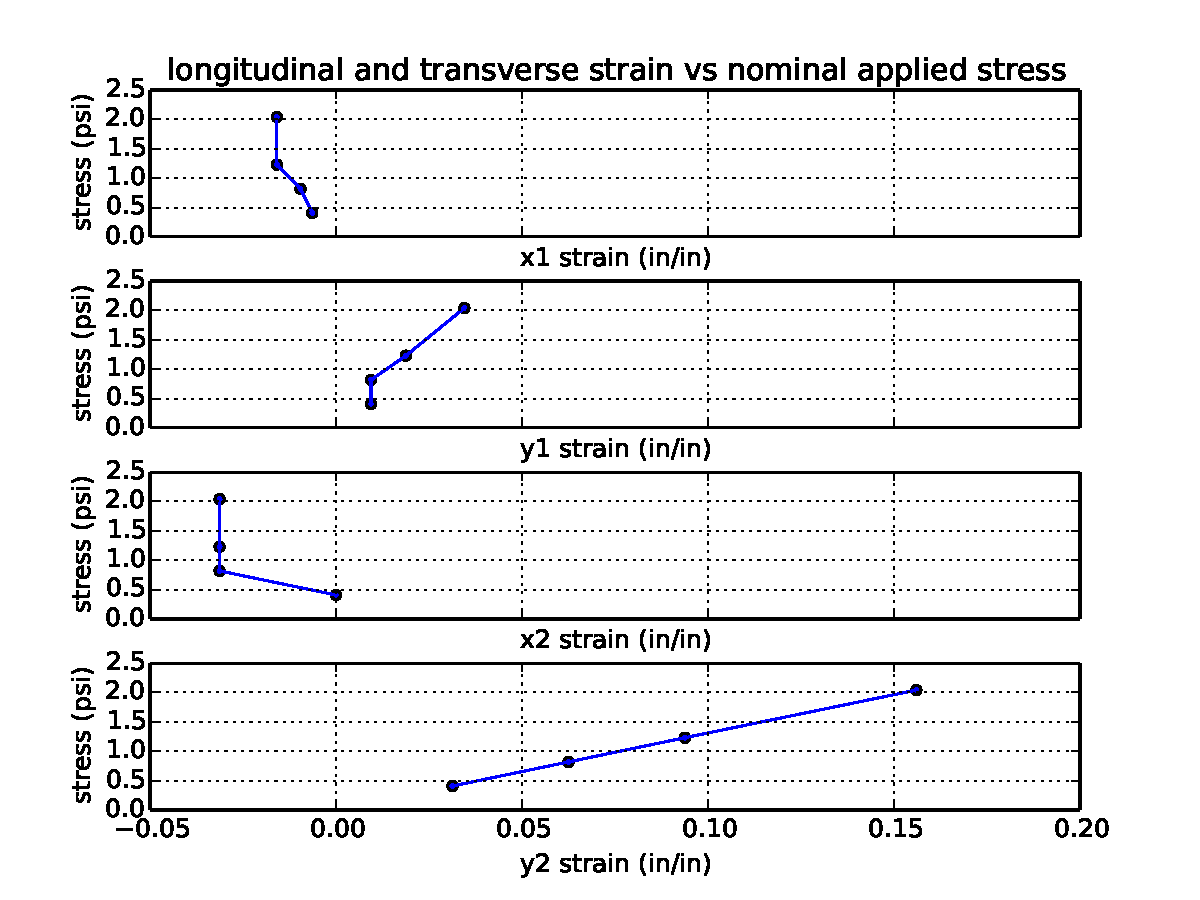
\includegraphics[width=250pt]{graph_p4.pdf}
\caption{A plot of the longitudinal and transfverse strain vs nominal applied stress. All four subplots share the same axis values (x,y). There were four test points for each subplot; these represent 10, 20, 30, and 50 lb weights being used.}
\end{figure}

\item[5) What is the ratio between the highest tensile stress and the average longitudinal tensile stress, known as the “stress
concentration factor?” Stress concentration can be easily obtained from your plots using a vertical line connecting
two data sets for locations 1 and 2.]
Come back to this

\item[6) Using your data from the transparent photoelastic plate sample, rank the relative stress concentration at all four (4)
non-circular openings from highest to lowest. Explain your results. Why should the shape of a “stress-raiser” matter?]
The holes with the smaller radi of curviture have the highest number of cycles and thus contain more stress in them. The holes with large radi of curviture (second sheet, bottom) have a smaller number of cycles and less stress. As a result, we must take into consideration the shape of holes/cracks that form in materials as the stress can vary greatly.
\begin{figure}[H]
\centering
\begin{tabular}{c | c | c}
Rank & \# cycles & location \\ \hline
1 & $2 \frac{2}{3}$ & first sheet, top \\ \hline
1 & $2 \frac{2}{3}$ & second sheet, top \\ \hline
3 & $2 \frac{1}{3}$ & first sheet, bottom \\ \hline
4 & $1 \frac{2}{3}$ & second sheet, bottom \\ \hline
\end{tabular}
\caption{ranking for transparent photoelastic sheets. Cycles represents the number of color changes, i.e. yellow $\rightarrow$ red $\rightarrow$ green is one complete cycle.}
\end{figure}

\item[7) When a uniaxial stress $\sigma_y$ is applied to a material (Fig. 8), there are resulting elastic strains ($\epsilon_y$ and $\epsilon_x$ ) along both the y and x directions that are proportional to the applied stress, where E is Young's Modulus and $\upsilon$ is Poisson's Ratio. Write down the expressions for $\epsilon_y$ and $\epsilon_x$ when the same part is subject to a biaxial stress state, that is, both $\sigma_x$ and $\sigma_y$, as illustrated in Fig. 9. Hint: the principle of “superposition” applies here. Begin by writing the equations for the strains when only $\sigma_x$ is applied, add the equations for the strains when only $\sigma_y$ is applied (above), and simplify.]
\begin{equation}
\begin{split}
\epsilon_x &= \frac{\sigma_x}{E} \Rightarrow -\epsilon_y \upsilon = \frac{\sigma_x}{E} \Rightarrow \epsilon_y = \frac{-\sigma_x}{\upsilon E} \\
\epsilon_y &= \frac{\sigma_y}{E},\, \epsilon_x = \frac{-\upsilon \sigma_y}{E},\, \epsilon_x = \frac{\sigma_x}{E},\, \epsilon_y = \frac{-\sigma_x}{\upsilon E} \\
&\text{Add the two equations for both $\epsilon_x$ and $\epsilon_y$.} \\
2\epsilon_y &= \frac{-\sigma_x}{\upsilon E}  + \frac{\sigma_y}{E}, \, 2\epsilon_x = \frac{\sigma_x}{E} + \frac{-\upsilon \sigma_y}{E} \\
&\text{simplify,} \\
\epsilon_y &= \frac{1}{2E}(\sigma_y - \frac{\sigma_x}{\upsilon}),\,\, \epsilon_x = \frac{1}{2E}(\sigma_x - \frac{\upsilon}{\sigma_y})
\end{split}
\end{equation}
\begin{center}
\begin{tikzpicture}
\node at (5,5) {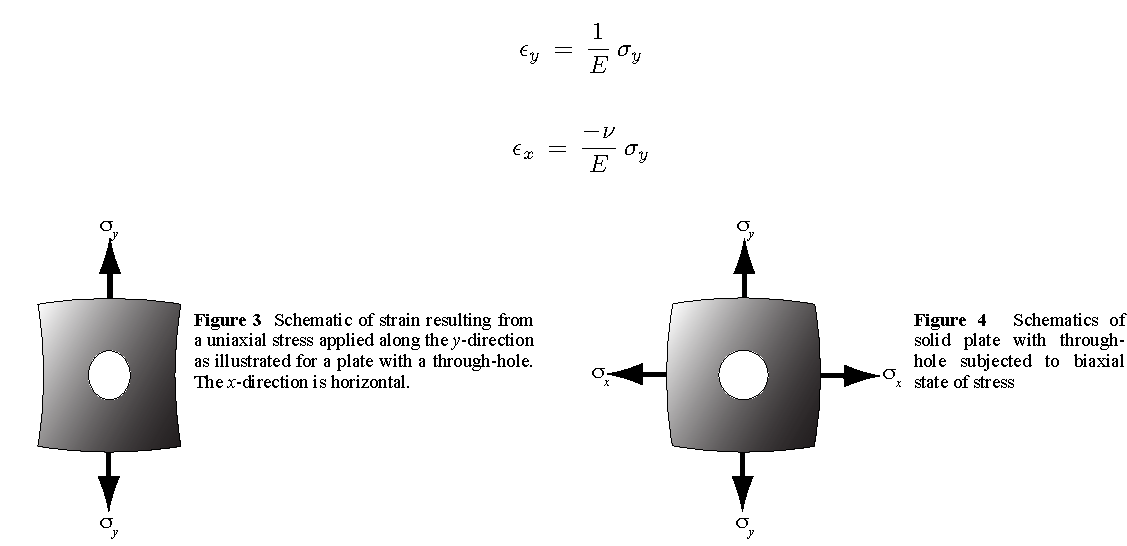
\includegraphics[width=400pt]{diagram22.pdf}};
\draw [fill=white,thick,white] (1.1,4.35) rectangle (1.3,4.5);
\draw [fill=white,thick,white] (10.15,4.35) rectangle (10.3,4.5);
\node at (1.2,4.445) {\footnotesize{8}};
3\node at (10.3,4.445) {\footnotesize{9}};
\end{tikzpicture}
\end{center}
\end{description}
%----------------------------------------------------------------------------------------
%	SECTION 4
%----------------------------------------------------------------------------------------

\section{Conclusions}


%----------------------------------------------------------------------------------------
%	SECTION 5
%----------------------------------------------------------------------------------------

\section{References}

%----------------------------------------------------------------------------------------
%	SECTION 6
%----------------------------------------------------------------------------------------

% Nothing right now

%----------------------------------------------------------------------------------------
%	BIBLIOGRAPHY
%----------------------------------------------------------------------------------------

\bibliographystyle{apalike}

\bibliography{sample}

%----------------------------------------------------------------------------------------


\end{document}
